
In this chapter, the described model is applied to a 4.62 kW grid-connected
PV system located in Bavaria, Germany (48.32° N, 11.91° E) and analyzed. The system
consists of 14 identical monocrystalline modules installed
with the same orientation of 28° tilt and 50° azimuth on the roof of a
small building. Two strings of seven modules each are connected separately
to an inverter with two independent MPPT inputs, allowing each string to
operate at its individual maximum power point. The required module parameters
at Standard Test Conditions (STC) were obtained from the manufacturer's datasheet
and are listed in Table \ref{tab:PV_system_surfclub_module_parameters}.
As graphical data of the I-V curve at STC were lacking, the absolute
values of the reciprocals of the slopes were estimated using Equations
\ref{eq:Estimation_of_Rso} and \ref{eq:Estimation_of_Rsho}. As
the panels face predominantly lake water and partly
green grass, a surface ground albedo of \(\rho = 0.1\) was assumed.
This value results from a weighted interpolation between the
recommended values for the ocean (0.06) and fresh grass (0.26),
with respective weighting factors of 4/5 and 1/5 \cite{OceanAlbedoWebsite}.
Meteorological measurements at 10-minute intervals were obtained from
two weather stations listed by the German Meteorological Office (DWD).
Air temperature, air pressure \cite{DWD_munich_airport_temperature_and_pressure},
and wind speed \cite{DWD_munich_airport_wind_speed} were recorded at a
nearby airport located 7.85 km from the site. Global and diffuse
horizontal irradiance \cite{DWD_weiherstephan_irradiance} were
measured with a Kipp \& Zonen CM11 Pyranometer situated 18.39 km from
the site. The predicted power values P were derived from the simulated
power values of the model \(P_{\text{model}}\) using the following equation:

\begin{equation}
    P = \min \bigl\{ P_{\text{model}}, c_{\text{max,DC}} \bigr\} \bigl(1 - f_{\text{decay}}(x_{\text{years}})\bigr)
    \label{eq:Power_prediction_from_the_model_output}
\end{equation}

\noindent
Here, \(c_{\text{max,DC}}\) is the historical maximum of the
measured DC power of the array, and \(f_{\text{decay}}(x_{\text{years}})\)
represents the decay factor after \(x_{\text{years}}\) of operation.
The constant \(c_{\text{max,DC}}\) is used to prevent overestimation of the
generated power as historical data are available and cover the
expected range of operating conditions. According to the datasheets,
the decay is specified for the expected lifetime of the PV modules,
in our case, a 20 \% reduction over 25 years. For simplicity, the decay factor
is assumed to be:

\begin{equation}
    f_{\text{decay}}(x_{\text{years}}) = \frac{0.2}{25} \, x_{\text{years}}
\end{equation}

\noindent
Other approaches can be adopted as well, but they require additional information \cite[p. 92]{Dolora2015}.

Two commonly used error measures for evaluating the accuracy of a
model are the relative mean bias error (rMBE) and the relative mean
absolute error (rMAE). These error measures are defined as:

\begin{align}
    \text{rMBE} &= \frac{1}{n} \sum_{i=1}^{n} \frac{\hat{y_i} - y_i}{y_i} \\
    \text{rMAE} &= \frac{1}{n} \sum_{i=1}^{n} \left| \frac{\hat{y}_i - y_i}{y_i} \right|
\end{align}

\noindent
Here, \(n\) is the number of data points, \(y_i\) are the observed values,
and \(\hat{y}_i\) are the predicted values. The rMAE measures how much the
predicted values differ from the observed values on average, expressed as a percentage
of the observed values. The rMBE measures the systematic error (bias) of
the predictions. While a positive rMBE indicates that the model tends
to overestimate the observed values, a negative rMBE indicates that the
model tends to underestimate them.

The physical model presented in Section \ref{sec:Five_parameter_model} has been shown
to accurately describe the I-V curves of different module types \cite{LoBrano, Orioli}
under various operating conditions. These studies validated their models using
their own measurements, thereby avoiding the discrepancies that can arise
when estimating operating conditions from meteorological data. Hence,
it can be expected that the model provides accurate generation predictions
if the true operating conditions are available. In general, PV forecasting
models use predicted meteorological
data from which, in the case of physical models, the operating conditions are
estimated. Due to the variable nature of the weather, these estimates are likely
to result in operating conditions that deviate from the actual conditions.
Similarly, when meteorological measurements are used where the instruments are
located several kilometers away from the site, as in this case, deviations from
the actual operating conditions should be expected.
Nevertheless, it may be possible to confirm the reliability of the model by
comparing the estimated power output of the PV system with the actual measured
data for time periods during which deviations in the weather conditions are
expected to be small. For this reason, the accuracy of the model was determined
for seven clear-sky days during periods when the modules were not shaded. The
time periods were determined by imposing the condition that the solar azimuth
angle was greater than 30°, the last angle at which the modules were potentially
shaded by surrounding trees. This condition resulted in time windows ranging
from shortly after midday to sunset. The results are reported in Table
\ref{tab:Performance_analysis_sunny_days}. As mentioned in \cite{Iheanetu2022},
physical models can achieve high accuracy in stable weather conditions, which,
at least for the conditions considered above, seems to be confirmed by the
relatively low relative mean absolute error (rMAE) ranging between 3.39 \%
and 7.82 \%. Interestingly, these conditions can also be leveraged to estimate the PV array's
tilt angle, a parameter that may be unknown in real-world applications, unlike the
more readily accessible geographical coordinates and azimuth of the PV array.
The latter variables can often be determined from the site's address, elevation
maps, and satellite imagery that account for magnetic declination \cite[p. 92]{Mayfield}.
Figure \ref{Surfclub_surface_tilt_and_average_rMAE.png} displays the averaged rMAEs
for the considered conditions across varying surface tilts. The shape of the curve
clearly indicates the region of the true PV array tilt of 28°, with minimal averaged
rMAEs centered around the curve's minimum at a tilt of 30°.

The presented model simulates the generated power
based on estimated operating conditions derived from meteorological measurements.
It is observed that, to a large extent, the generated power
mimics the behavior of the measured global horizontal irradiance values.
Figure \ref{fig:Surfclub_estimated_power_vs_GHI_collection} shows the estimated
power and measured global horizontal irradiance for three
different days. These plots clearly illustrate the one-to-one correspondence
between the spikes and dips in the curves of irradiance and power values.
Furthermore, the estimated power values seem to correspond to appropriately
scaled values of the measured global horizontal irradiance. The scaling
factor is higher during the day when the orientation of the modules is
towards the Sun, which is captured by the transposition model, and lower
during the morning and evening. For this reason, it can be foreseen that
the more the meteorological input deviates from the true conditions, the
greater the deviation between the estimated power values and the measured
power values. These considerations can be seen in Figure
\ref{fig:Surfclub_estimated_power_vs_measured_collection}, which compares
the measured power values with the estimated power values for the same
three days. As expected, the estimated power does not perfectly match
the measured power values. The predicted power values after 3 p.m. on
the first day (a) follow the smooth decline of the measured irradiance
values, whereas the fluctuations in the decline of the measured power
values indicate passing clouds between the Sun and the PV system.
Similarly, the discrepancies between spikes in predicted and measured
power between midday and afternoon on the second day (b) illustrate
the delayed movement of passing clouds. The spikes in the predicted power
observed between morning and midday on the third day (c) likely result
from direct sunlight incident on the irradiance sensor, while the measured
power remains low due to partial shading of the PV system by surrounding
trees during this period. The last two figures exclude the cut-off of
overestimated power by \(c_{\text{max,DC}}\) for the sake of comparison,
as introduced in Equation \ref{eq:Power_prediction_from_the_model_output}.

Finally, the accuracy of the model was evaluated over a period of
166 days between May 7 and October 19, 2024. Data was available
for 154 of those days. The rMBE and rMAE were calculated to be
8.92 \% and 56.73 \%, respectively. The positive rMBE suggests
that the model tends to overestimate the power output, which is
expected because the PV system is shaded by large trees during
the morning hours, a factor not accounted for in the model.
The rMBE drops to 2.74 \% when the periods during which the
surrounding trees are between the Sun and the PV system are
excluded from the analysis. The remaining positive rMBE may
be partly explained by the fact that the PV system's output
is limited by a certain threshold that appears to depend
on the operating conditions. This can be observed in Figure
\ref{fig:Surfclub_DC_output_comparison}, and for many other days,
where the measured output flattens out once a certain power
level is reached. This phenomenon is partly accounted for by
the clipping introduced in Equation
\ref{eq:Power_prediction_from_the_model_output}, but not entirely,
as the upper limit is not constant. 
Another possible source of error is an overestimation of the ground albedo.
This was likely the case in the present application, as the PV system faces
predominantly lake water and only partially green grass. This may have led
to an overestimation of reflected irradiance and thereby contributed to
the remaining positive bias. The high rMAE indicates that there is
significant discrepancy between the model's predicted power output
and the observed values.
This relatively high error can primarily be attributed to two factors.
First, the estimation of operating conditions from meteorological data
introduces uncertainties. In this thesis, meteorological measurements
were obtained from weather stations located approximately 7.85 km and
18.39 km from the PV system. Since local weather conditions can vary
over such distances, the estimated input conditions likely
deviate from the actual conditions experienced by the PV modules.
Second, the model does not include shading analysis. As mentioned
earlier, the PV system is surrounded by large trees that cast shadows
on the modules from sunrise until midday. Because this shading is not
accounted for in the simulation, it leads to a systematic overestimation
of the power output during the shaded periods. These two factors,
together with the previously discussed causes of the positive rMBE,
are likely the main contributors to the high rMAE observed over the
full 166-day analysis period.

\begin{table}
    \centering
    \resizebox{\columnwidth}{!}{
        \begin{tabular}{llccccccc}
            \toprule
            \textbf{Manufacturer} & \textbf{Module Type} & \(V_{\text{oc}}\) (V) & \(I_{\text{sc}}\) (A) & \(V_{\text{mp}}\) (V) & \(I_{\text{mp}}\) (A) & \(\mu_{\text{I,sc}}\) (\%/K) & \(\mu_{\text{V,oc}}\) (\%/K) & \(\mu_{P_{\text{mp}}}\) (\%/K) \\
            \midrule
            Trina Solar & TSM-330 DE06M.08(II) & 40.6 & 10.4 & 9.76 & 33.8 & 0.05 & -0.29 & -0.37 \\
            \bottomrule
        \end{tabular}
    }
    \caption{\small Data for the evaluation of the model parameters.}
    \label{tab:PV_system_surfclub_module_parameters}
\end{table}

\begin{table}
    \centering
    \begin{tabular}{cccc}
        \toprule
        \textbf{Date} & \multicolumn{2}{c}{\textbf{Interval}} & \textbf{rMAE (\%)} \\
        \midrule
        06/25/2024 & 12:20 & 19:10 & 3.39 \\
        08/06/2024 & 12:40 & 18:40 & 5.02 \\
        08/11/2024 & 12:40 & 18:30 & 5.81 \\
        05/14/2024 & 12:20 & 18:40 & 5.91 \\
        08/24/2024 & 12:40 & 18:00 & 6.52 \\
        07/30/2024 & 12:40 & 18:40 & 6.78 \\
        07/29/2024 & 12:40 & 18:50 & 7.82 \\
        \bottomrule
    \end{tabular}
    \caption{\small The relative mean absolute error (rMAE) of the model for clear sky days and no shading.}
    \label{tab:Performance_analysis_sunny_days}
\end{table}

\begin{figure}
    \centering
    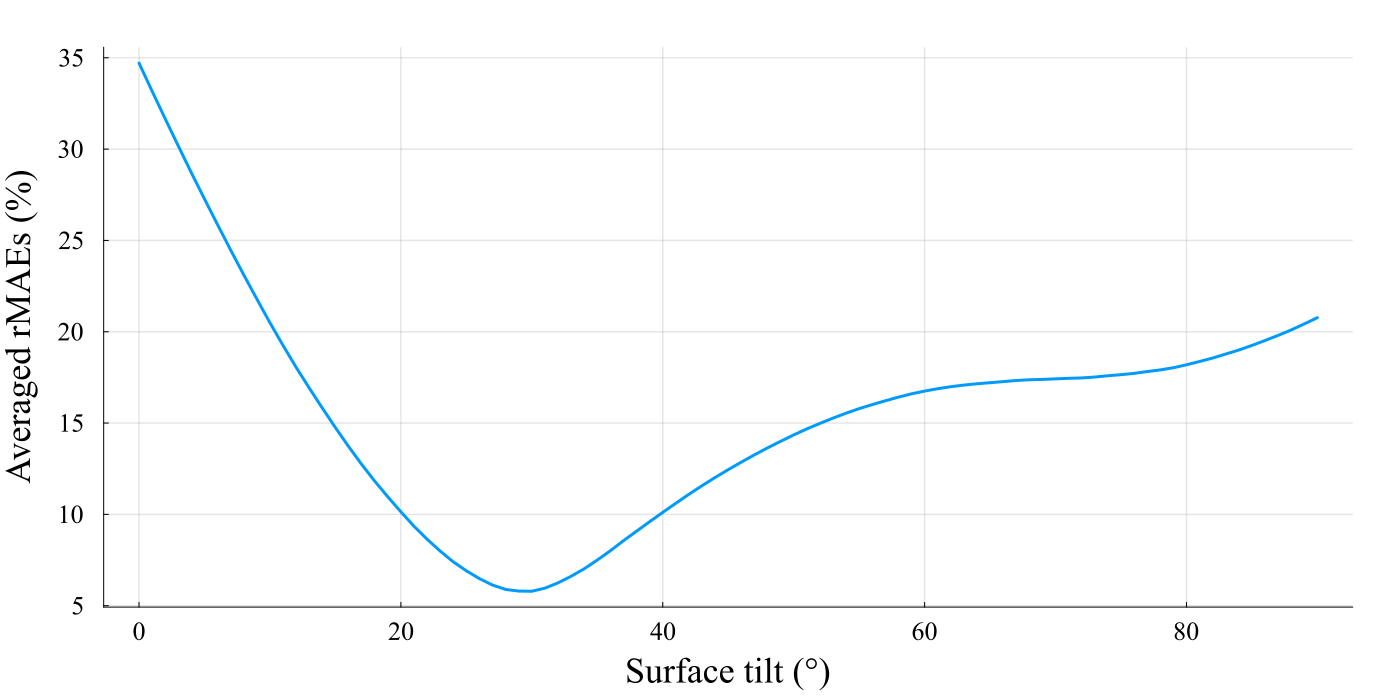
\includegraphics[scale=0.3075]{Surfclub_surface_tilt_and_average_rMAE.png}
    \caption{\small Averaged relative mean absolute errors for clear sky days and no shading with varying surface tilt.}
    \label{Surfclub_surface_tilt_and_average_rMAE.png}
\end{figure}

\begin{figure}
    \centering
    \subfloat[\centering][05/24/2024]{{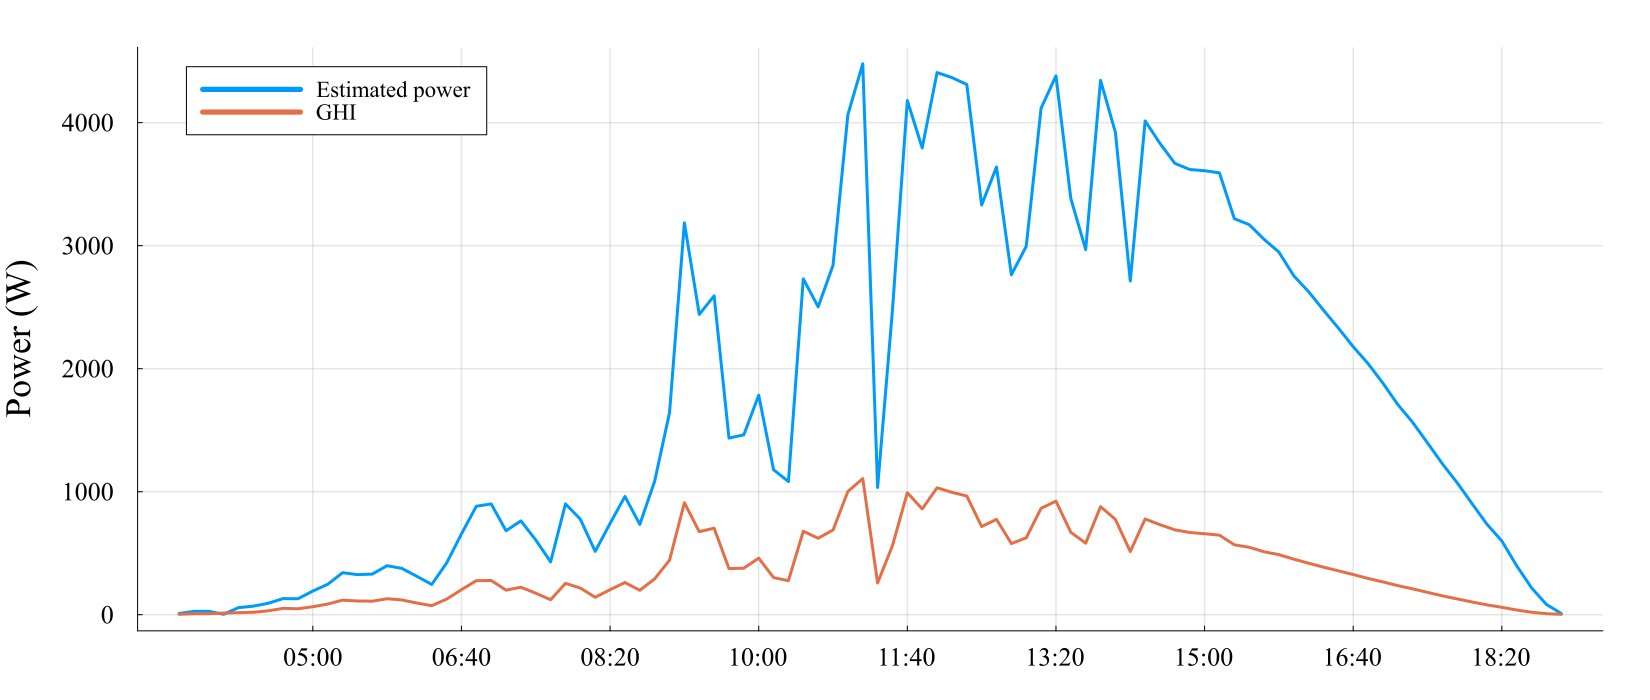
\includegraphics[scale=0.255]{Surfclub_estimated_power_vs_GHI_2024_05_24.png}}} \\
    \subfloat[\centering][07/02/2024]{{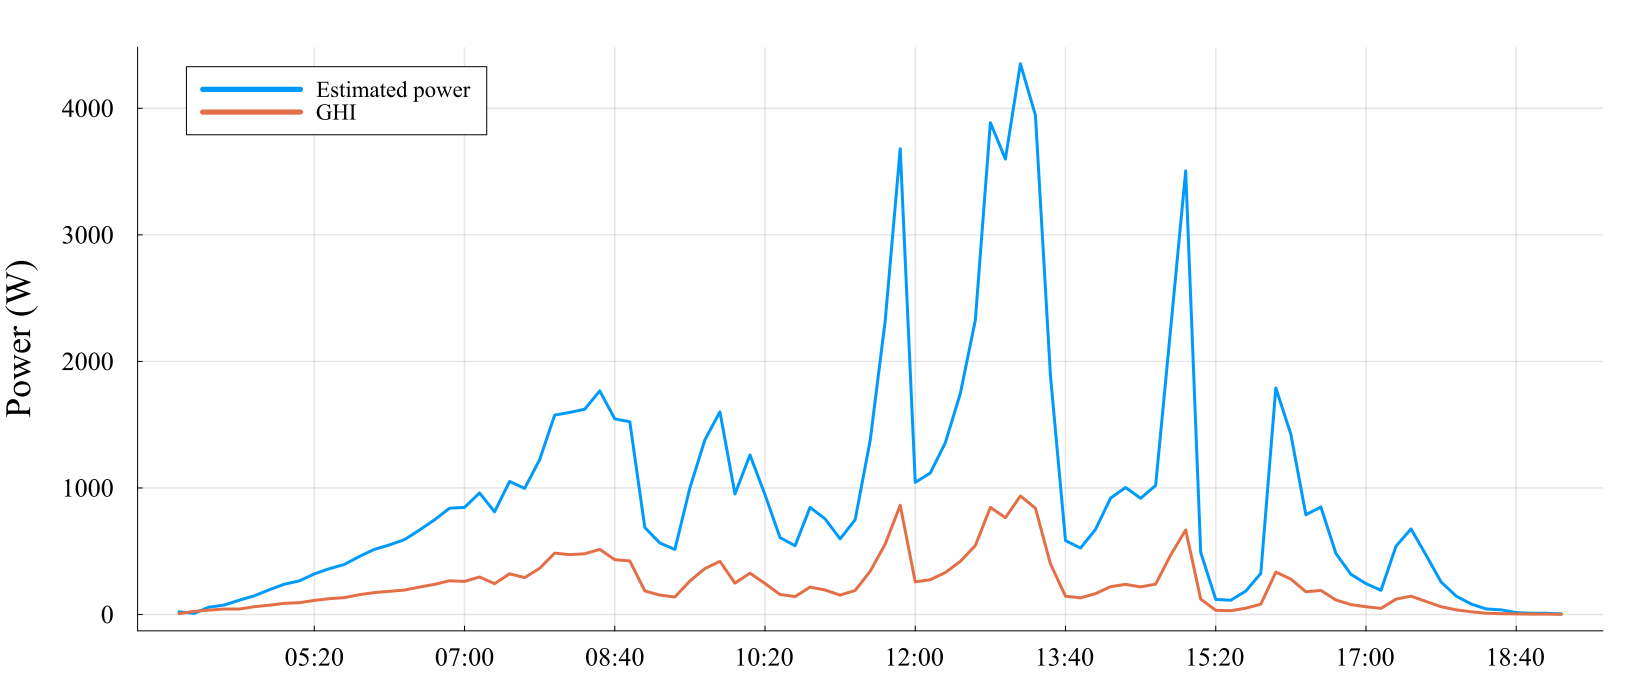
\includegraphics[scale=0.255]{Surfclub_estimated_power_vs_GHI_2024_07_02.png}}} \\
    \subfloat[\centering][10/08/2024]{{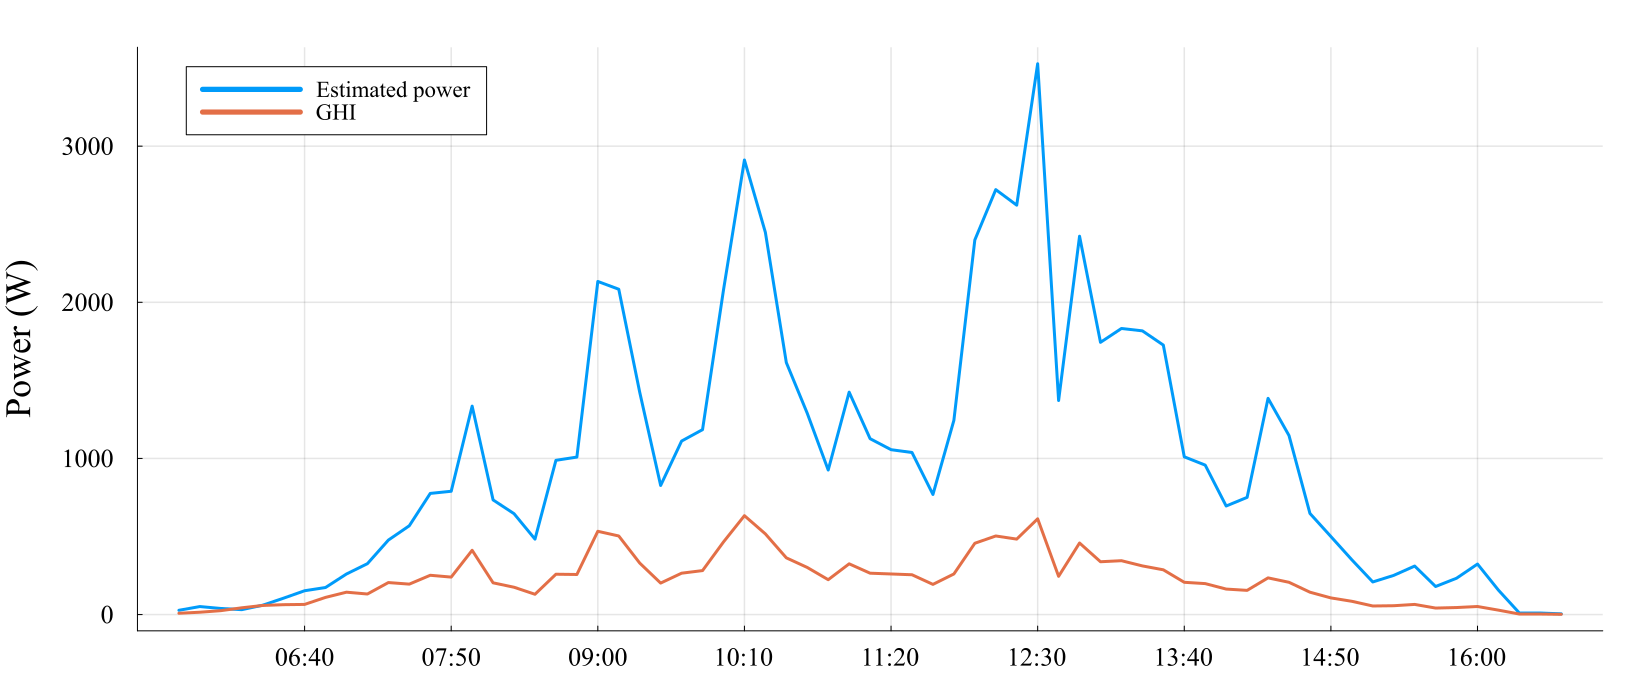
\includegraphics[scale=0.255]{Surfclub_estimated_power_vs_GHI_2024_10_08.png}}}
    \caption{\small Estimated power output of the model and measured global horizontal irradiance for different days of the year.}
    \label{fig:Surfclub_estimated_power_vs_GHI_collection}
\end{figure}

\begin{figure}
    \centering
    \subfloat[\centering][05/24/2024]{{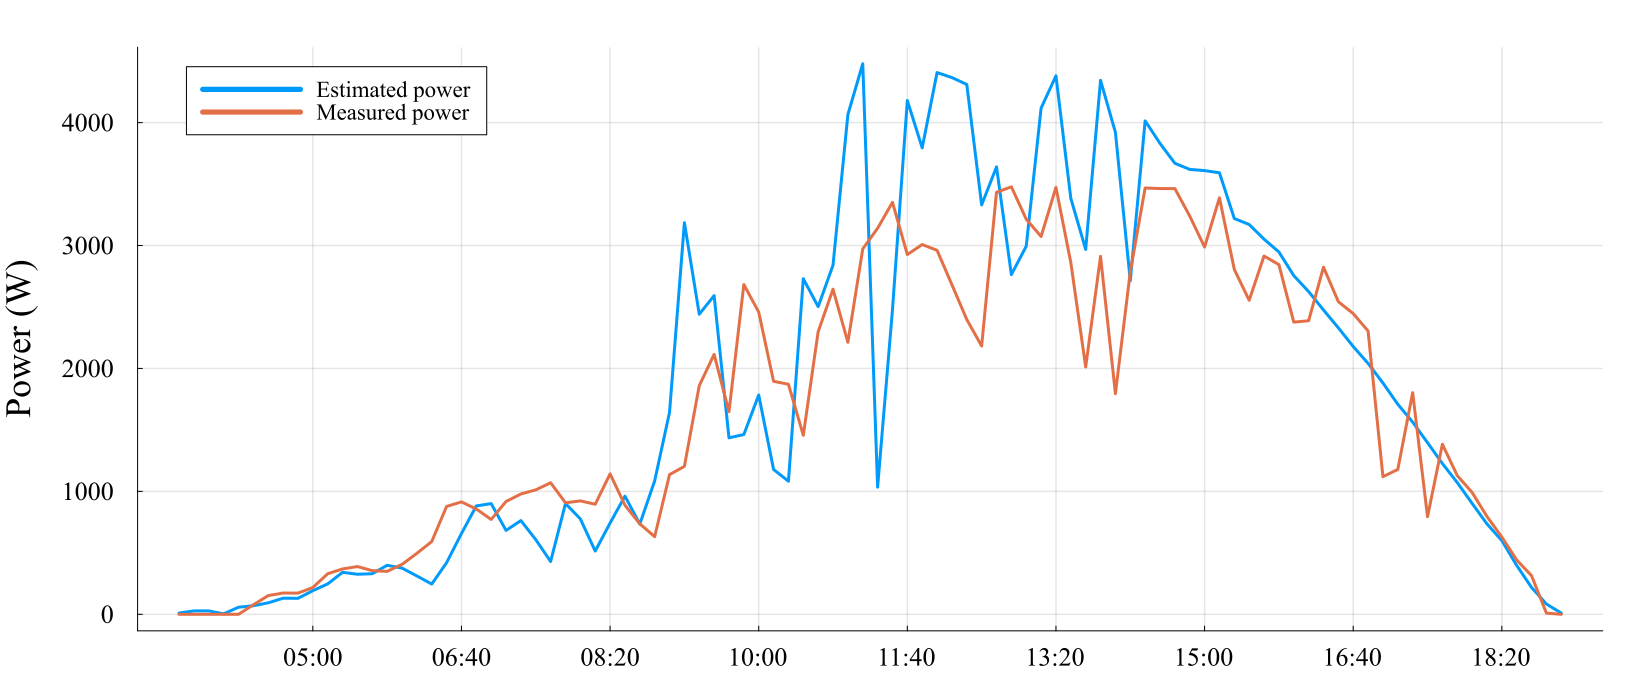
\includegraphics[scale=0.255]{Surfclub_estimated_power_vs_measured_2024_05_24.png}}} \\
    \subfloat[\centering][07/02/2024]{{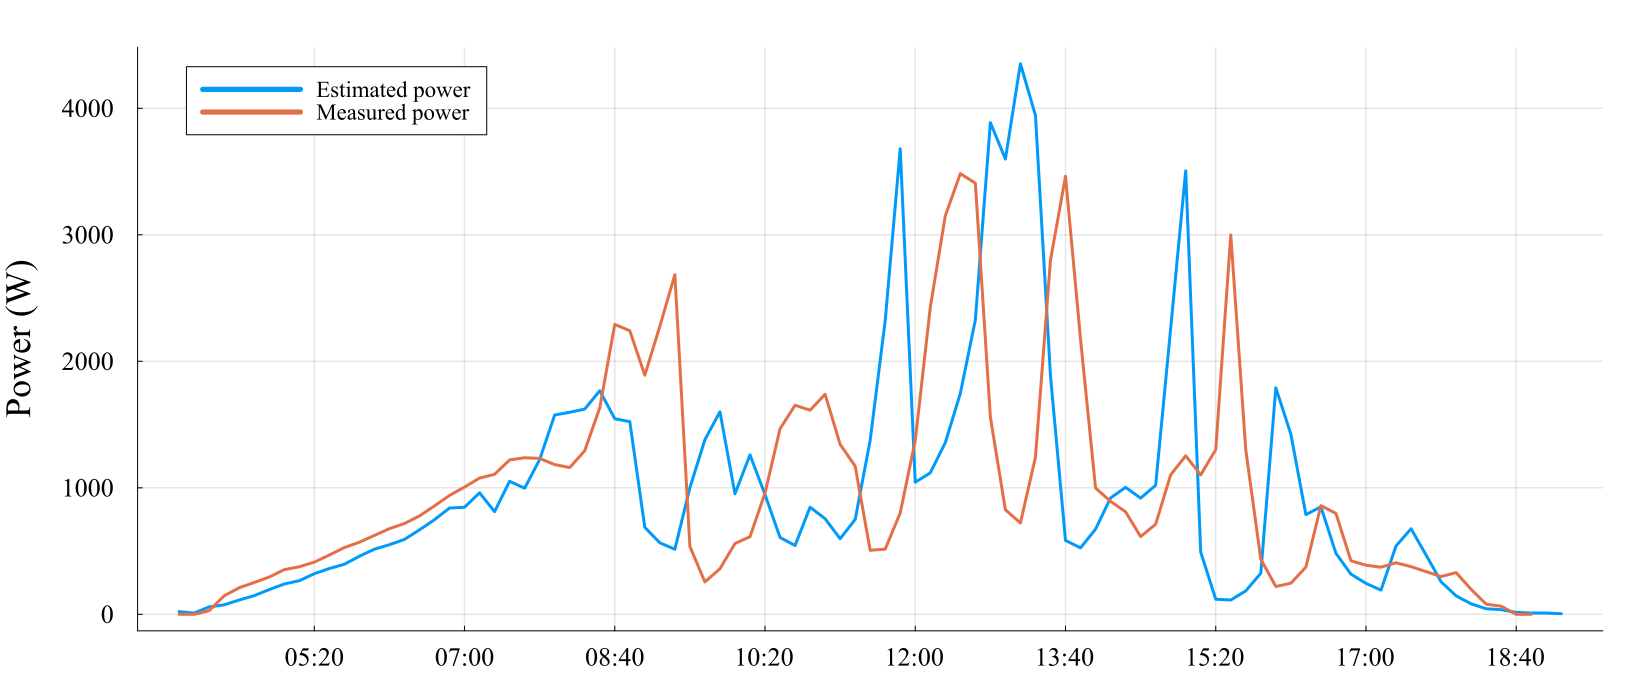
\includegraphics[scale=0.255]{Surfclub_estimated_power_vs_measured_2024_07_02.png}}} \\
    \subfloat[\centering][10/08/2024]{{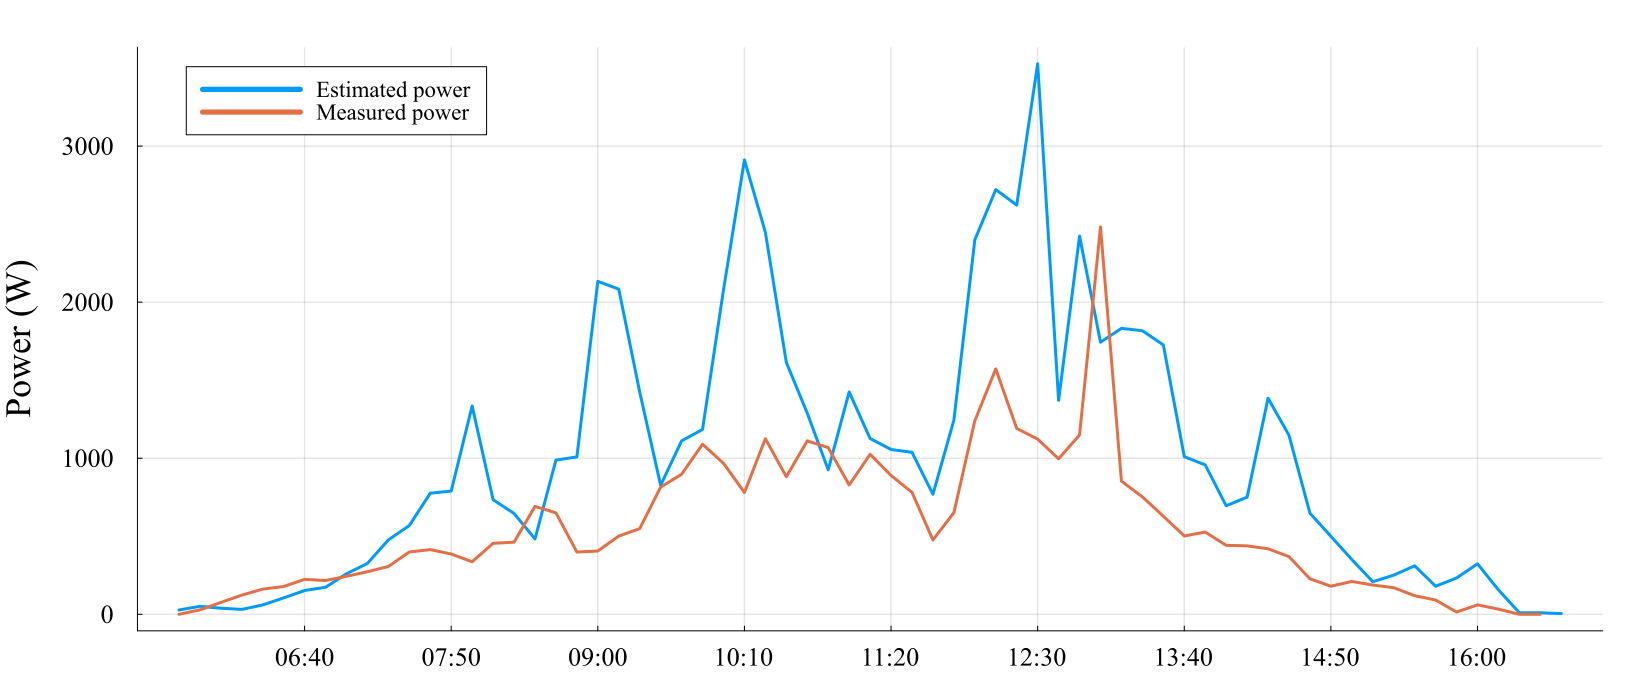
\includegraphics[scale=0.255]{Surfclub_estimated_power_vs_measured_2024_10_08.png}}}
    \caption{\small Estimated power output of the model and measured power output for different days of the year.}
    \label{fig:Surfclub_estimated_power_vs_measured_collection}
\end{figure}
